%%%%%%%%%%%%%%%%%%%%%%%%%%%%%%%%%%%%%%%%%%%%%%%%%%%%%%%%%%%%%%%%%%%%%%%%%%%%%%%%%%%%%%%%%%%%%
%%									Chapitre Introduction
%%%%%%%%%%%%%%%%%%%%%%%%%%%%%%%%%%%%%%%%%%%%%%%%%%%%%%%%%%%%%%%%%%%%%%%%%%%%%%%%%%%%%%%%%%%%%
%\addcontentsline{toc}{part}{Introduction Générale}
%\markboth{Introduction Générale}{}
\chapter{Présentation d’Excel}

\section*{}
Excel est un tableur créé par la société Microsoft conçu sous forme de cellules. Il est issu de la suite du logiciels bureautiques Office. Il est un logiciel de calcul  ainsi que de traitement de texte.
\section{Vocabulaire}  
 	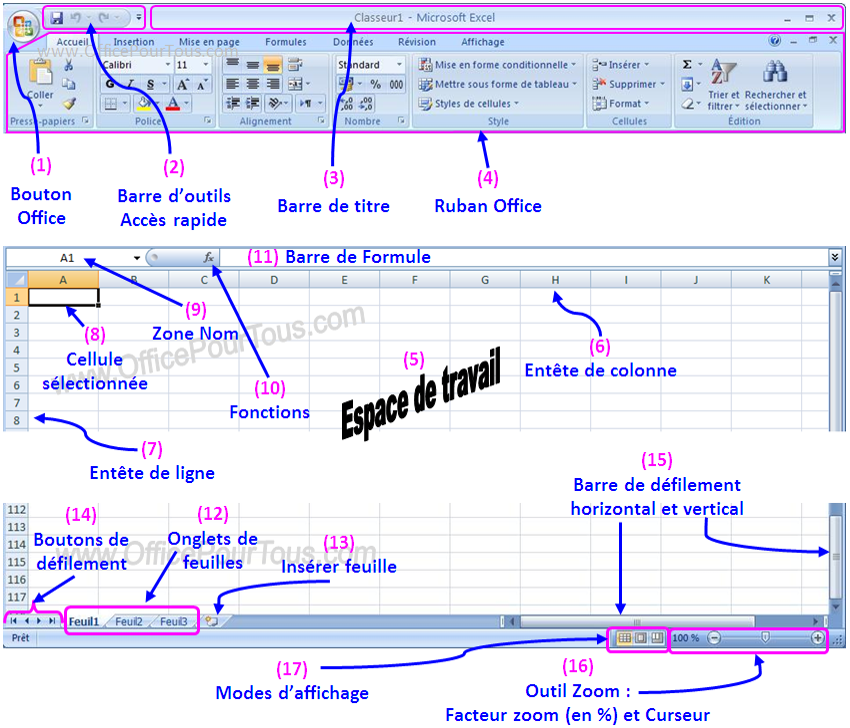
\includegraphics[width=\linewidth]{img/interface}

\begin{definition}[Adressage]
l'adressage est le point de repérage d’une cellule.\\
Une cellule est repéré par deux 2 symboles:  un nombre et une lettre.
\begin{itemize}
	\item La lettre permet de repérer une cellule verticalement.
	\item Le nombre permet de repérer une cellule horizontalement. 
\end{itemize}
\begin{center} 
	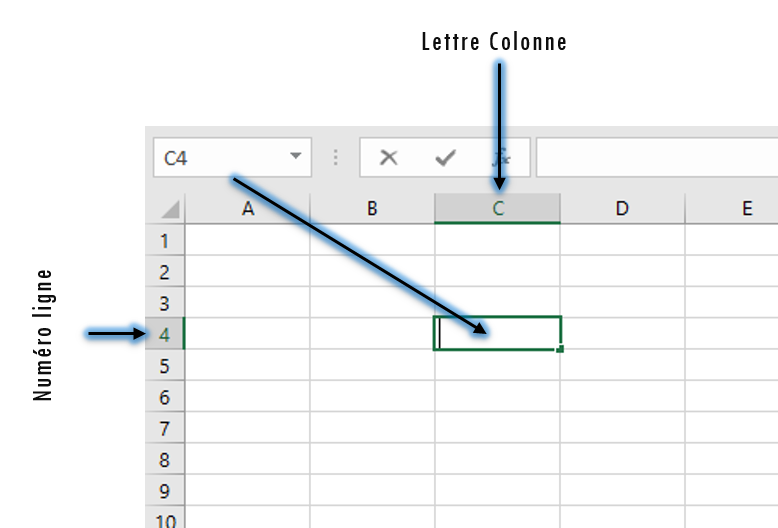
\includegraphics[scale=0.2,width=\linewidth]{img/adressage} 
	\captionof{figure}{Adressage d'une cellule} \label{rdp}
\end{center}
\end{definition}

\begin{definition}[Ruban]
	Il regroupe les fonctionnalités du logiciel, celui-ci évolué  graphiquement avec les mise à jours.\\
	Le ruban est composé d’onglet qui dont de gauche à droite: Accueil, Insertion, Mise en page, formules, Données, Révision, Affichage.
	Ainsi chaque onglet est subdivisé en groupe de même famille.
	\begin{center} 
		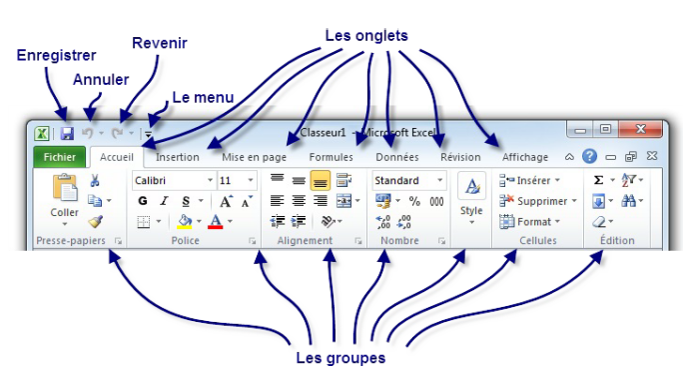
\includegraphics[scale=0.2,width=\linewidth]{img/ruban} 
		\captionof{figure}{Ruban} \label{rdp}
	\end{center}
\end{definition}

	\begin{wrapfigure}{r}{0.2\textwidth}
		\vspace{-2pt}
		\begin{center}
			
\includegraphics[width=0.2\textwidth]{img/barre_access_rapide}
		\end{center}  
		\vspace{-2pt}  
	\end{wrapfigure}
\subsection*{}
\begin{definition}[Barre d'outils Accès rapide]
	
	Comme son nom l’indique, elle permet l'accès rapide aux fonctionnalités globalement utilisées d'Excel.
 
  \textbf{Raccourci clavier: }
 \begin{itemize}
 	\item Ctrl + S: Enregistrer votre document
 	\item Ctrl + C: Copier la cellule sélectionnée
 	\item Ctrl + V: Coller les éléments copier
 	\item Ctrl + S: Couper les éléments sélectionnée
 	\item Ctrl + Z: Annuler la dernière action
 	\item Ctrl + Y: Répéter la dernière action 
 	\item Ctrl + N:  création d'un nouveau fichier
 	\item Ctrl + P: Impression
 	\item Ctrl + O: Ouvrir un fichier existant 	
 \end{itemize}
\end{definition}
\begin{wrapfigure}{r}{0\textwidth}
 
\end{wrapfigure}
\subsection*{}
\begin{definition}[La barre de formules]
	la zone principale de la barre de formule permet d’afficher le contenu d’une cellule sélectionnée. Il peut contenir du texte, nombre, date, fonction ou formule…
	\paragraph{Insérer une fonction:}{le button fx permet d’insérer une fonction dans le calculs}
\end{definition}
\begin{center} 
	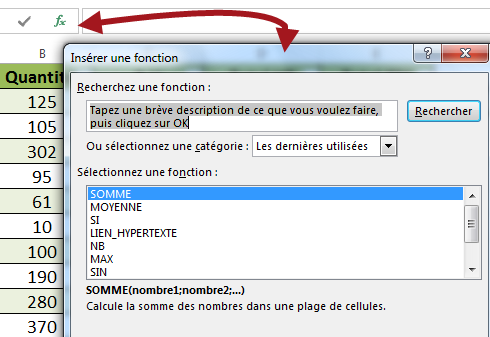
\includegraphics[scale=0.2,width=\linewidth]{img/barre_formule} 
	\captionof{figure}{Barre de Formule} \label{rdp}
\end{center}

\paragraph{Masquer ou afficher la barre de formule}{\hfill\\
 	\begin{enumerate}
 		\item Cliquez sur le menu Fichier => Options.
 		\item Dans la fenêtre qui s’affiche, cliquez sur Options avancées.
 		\item Dans la catégorie Afficher, décochez la case Afficher la barre de formule.
 		\item Validez enfin.
 	\end{enumerate}
 \begin{center} 
 	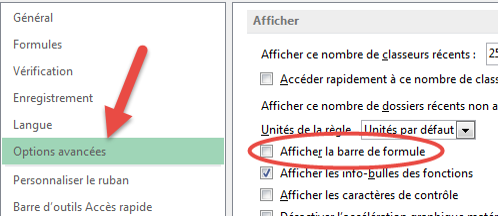
\includegraphics[scale=0.2,width=\linewidth]{img/Masquer_barre} 
 	\captionof{figure}{Masquer ou afficher la barre de formule} \label{rdp}
 \end{center}
}
\paragraph{Empêcher l’affichage des formules dans la barre de formule}{
	Lorsque vous aimez interdire à l’utilisateur de votre classeur Excel de voir les formules utilisées dans une cellule, vous devez faire deux choses :
	\begin{enumerate}
		\item Masquez votre cellule.
			\subitem Pour masquer votre cellule, sélectionnez-la et tapez Ctrl+Mj+\&
			\subitem Choisissez l’onglet Protection et cochez Masquer, puis cliquez sur OK.	
\begin{center} 
	\includegraphics[scale=0.2,width=0.5\linewidth]{img/masquer} 
	\captionof{figure}{Afficher-Masquer formule} \label{rdp}
	\end{center} 
\item Protégez votre feuille.
	\subitem Pour protéger votre feuille, cliquez sur l’onglet Révision puis sur Protéger la feuille.
	\subitem Entrez votre mot de passe et validez.
	\subitem Sélectionnez maintenant votre cellule et remarquez que la barre de formule n’affiche rien.
	
\end{enumerate}
}
\begin{definition}[Barre d'état]

\end{definition}
 \begin{center} 
	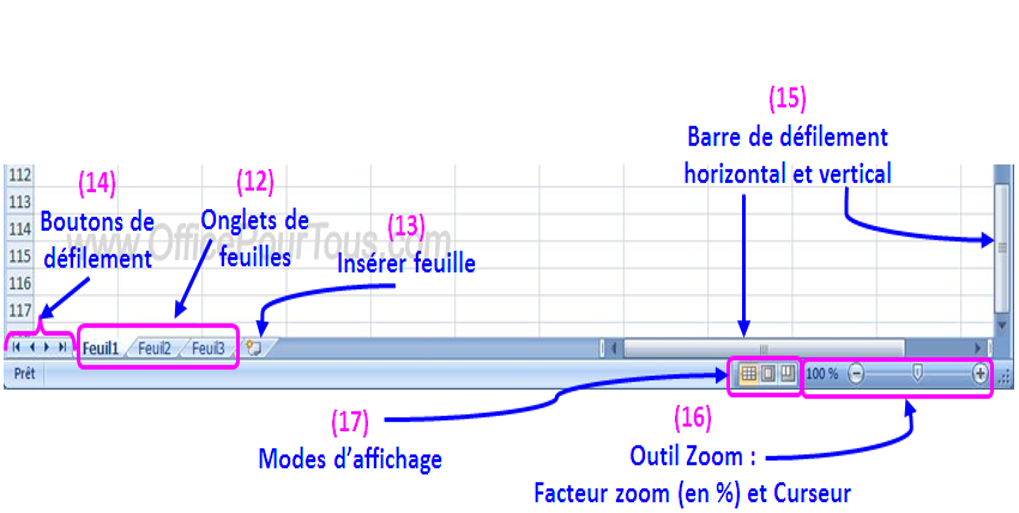
\includegraphics[scale=0.2,width=\linewidth]{img/barre_etat} 
	\captionof{figure}{Barre d'état} \label{rdp}
\end{center}


